\section{Resolved top tagger in 8\:\TeV\: Data}
\label{app:8TeV}

In this Appendix we compare the inputs and the output of the resolved top tagger, and the efficiency of the resolved top tagger in 8 TeV data and simulations. The level of agreement of the CVS output is not great (Fig. \ref{fig:jet12csv}). Other than that, we notice an overall fair agreement between data and simulations for all the top tagger input and output variables, as well as for efficiency and fake rates.

\begin{figure}[htbp]
	\centering
	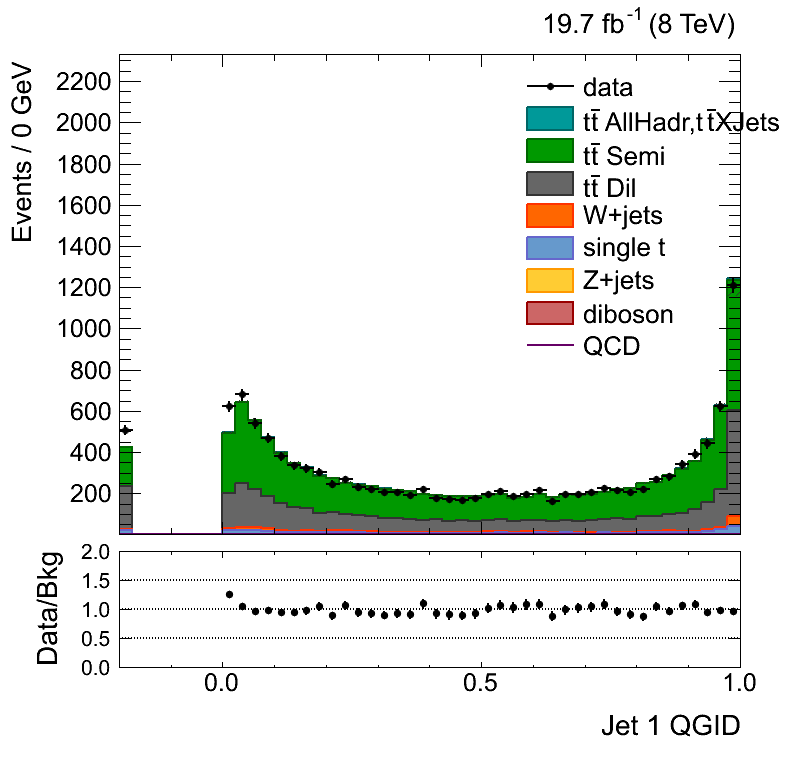
\includegraphics[width=0.48\textwidth]{figures/semilep_1tightmuo_resolved_3ormorejets_2ormorejetWPm_pfmetmore100_pfmtmore40_trigrequestonMC_17102015/res_hJet1qgid.png}
	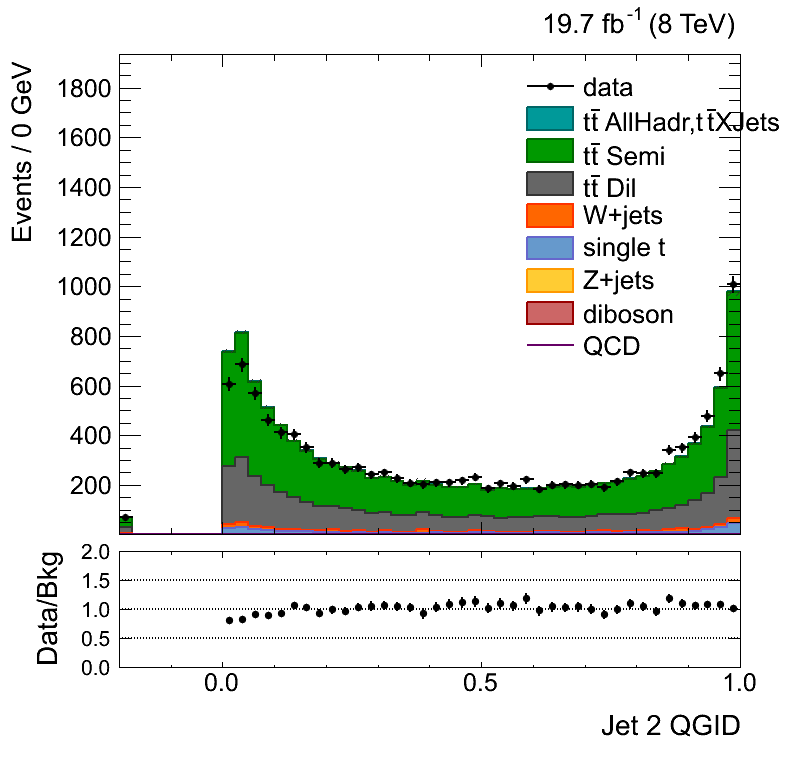
\includegraphics[width=0.48\textwidth]{figures/semilep_1tightmuo_resolved_3ormorejets_2ormorejetWPm_pfmetmore100_pfmtmore40_trigrequestonMC_17102015/res_hJet2qgid.png}
	\caption{Quark/gluon discriminant output in data and MC of the two jets in the triplet which maximizes the resolved tagger. The jet with the highest-CSV has not been considered.}
	\label{fig:qgid1213TeV}
\end{figure}

\begin{figure}[htbp]
	\centering
	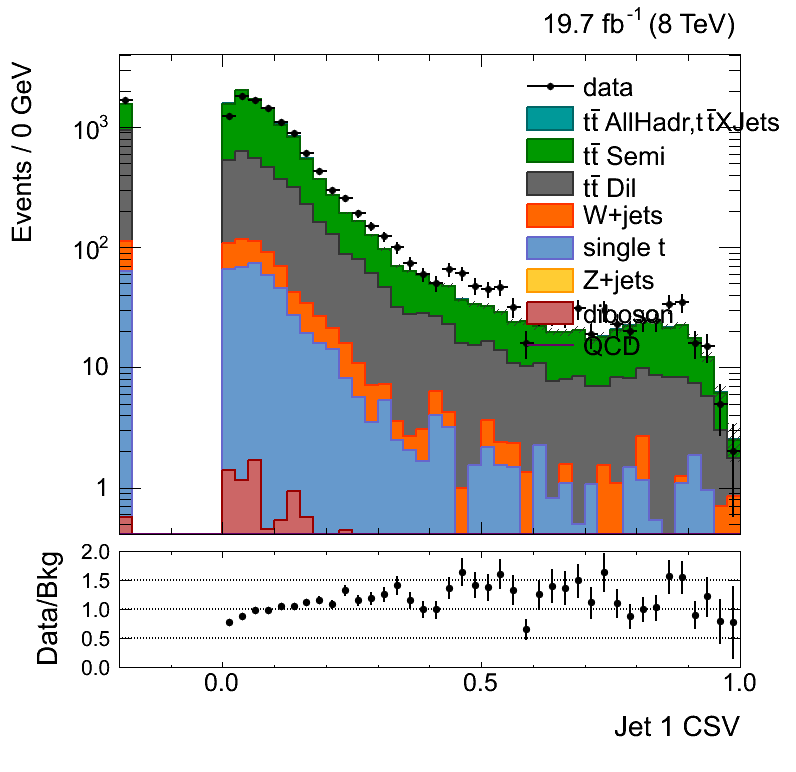
\includegraphics[width=0.48\textwidth]{figures/semilep_1tightmuo_resolved_3ormorejets_2ormorejetWPm_pfmetmore100_pfmtmore40_trigrequestonMC_17102015/res_hJet1csv.png}
	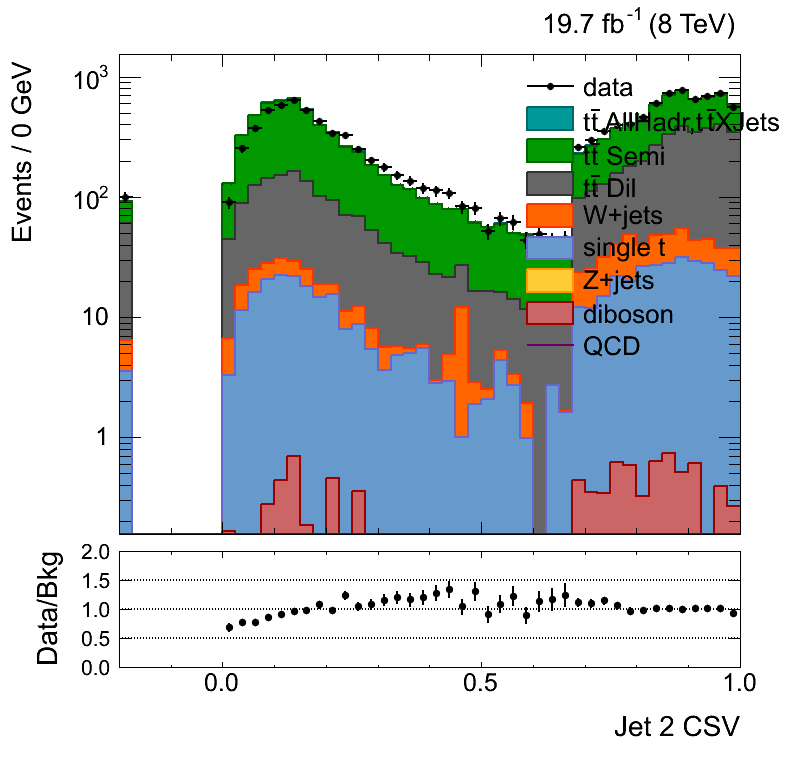
\includegraphics[width=0.48\textwidth]{figures/semilep_1tightmuo_resolved_3ormorejets_2ormorejetWPm_pfmetmore100_pfmtmore40_trigrequestonMC_17102015/res_hJet2csv.png}
	\caption{CSV output in data and MC of the two jets in the triplet which maximizes the resolved tagger. The jet with the highest-CSV has not been considered.}
	\label{fig:jet12csv}
\end{figure}

\begin{figure}[htbp]
	\centering
	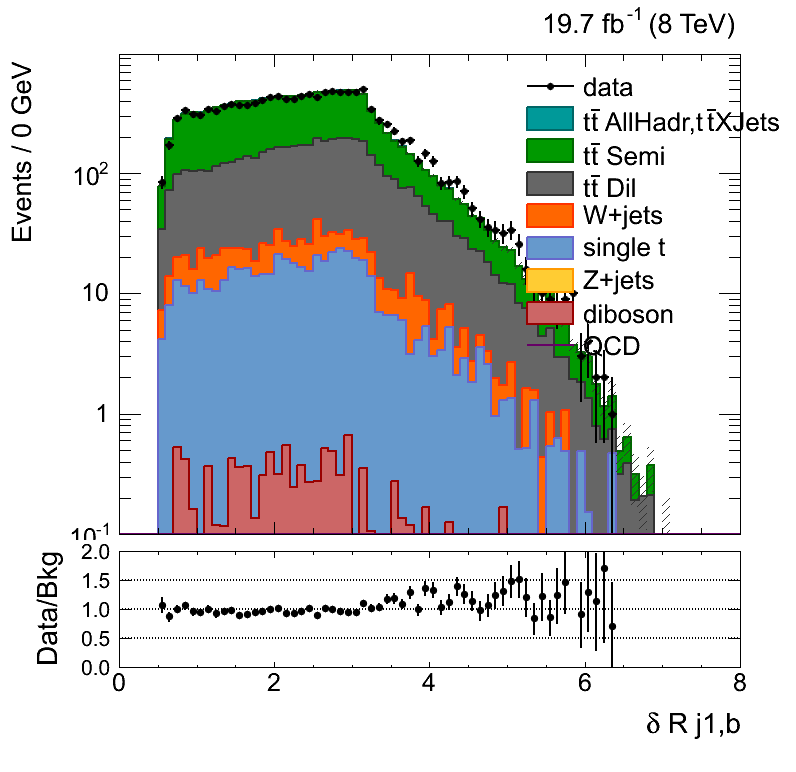
\includegraphics[width=0.48\textwidth]{figures/semilep_1tightmuo_resolved_3ormorejets_2ormorejetWPm_pfmetmore100_pfmtmore40_trigrequestonMC_17102015/hResBDTDRj1b.png}
	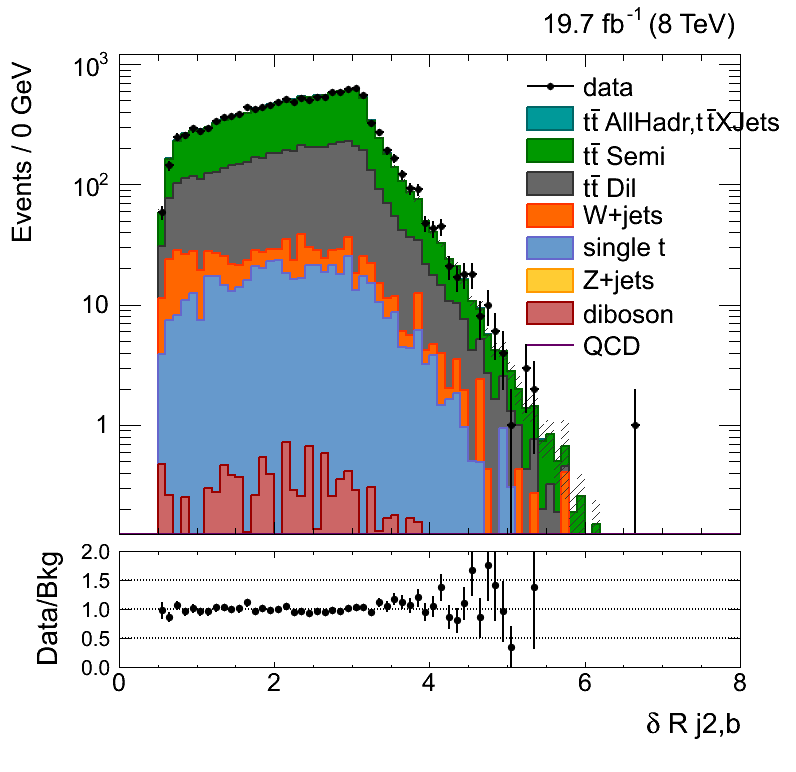
\includegraphics[width=0.48\textwidth]{figures/semilep_1tightmuo_resolved_3ormorejets_2ormorejetWPm_pfmetmore100_pfmtmore40_trigrequestonMC_17102015/hResBDTDRj2b.png}
	\caption{Data and MC comparisons for the $\Delta$ R between the first and the third jet (left), the second and the third jet (right) of the triplet which maximizes the resolved tagger. The jets have been ordered in decreasing CSV output.}
	\label{fig:dRj12b13TeV}
\end{figure}

\begin{figure}[htbp]
	\centering
	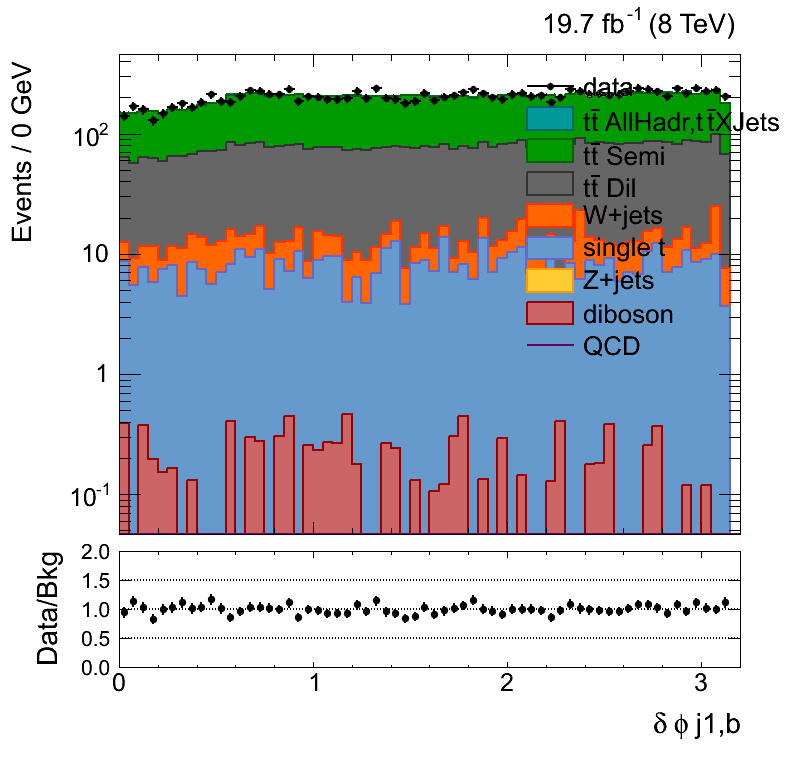
\includegraphics[width=0.48\textwidth]{figures/semilep_1tightmuo_resolved_3ormorejets_2ormorejetWPm_pfmetmore100_pfmtmore40_trigrequestonMC_17102015/hResBDTDPhij1b.png}
	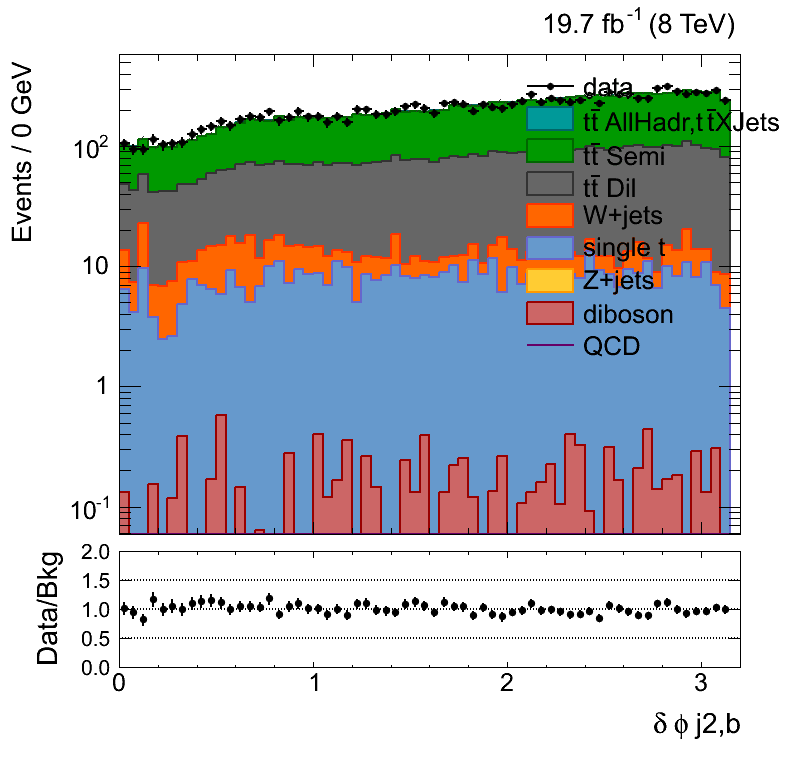
\includegraphics[width=0.48\textwidth]{figures/semilep_1tightmuo_resolved_3ormorejets_2ormorejetWPm_pfmetmore100_pfmtmore40_trigrequestonMC_17102015/hResBDTDPhij2b.png}
	\caption{Data and MC comparisons for the $\Delta \phi$  between the first and the third jet (left), the second and the third jet (right) of the triplet which maximizes the resolved tagger. The jets have been ordered in decreasing CSV output.}
	\label{fig:dphij12b13TeV}
\end{figure}

\begin{figure}[htbp]
	\centering
	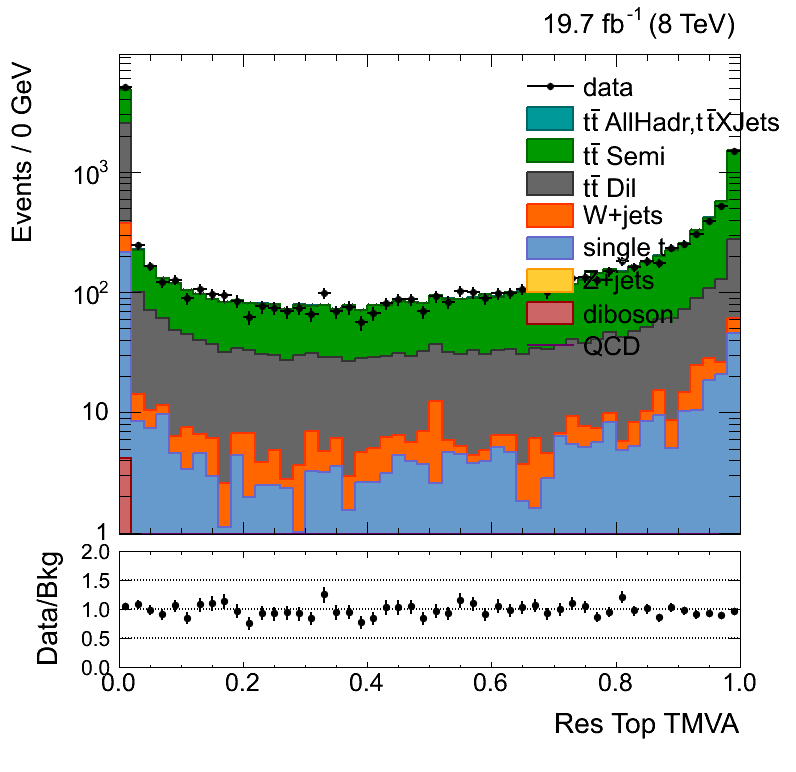
\includegraphics[width=0.48\textwidth]{figures/semilep_1tightmuo_resolved_3ormorejets_2ormorejetWPm_pfmetmore100_pfmtmore40_trigrequestonMC_17102015/hResProb.png}
	\caption{Fit probability in Data and MC. The fit probability variable has been described in Sec. \ref{subsec:sel_toptag_resolved}.}
	\label{fig:fitprob13TeV}
\end{figure}

\begin{figure}[htbp]
	\centering
	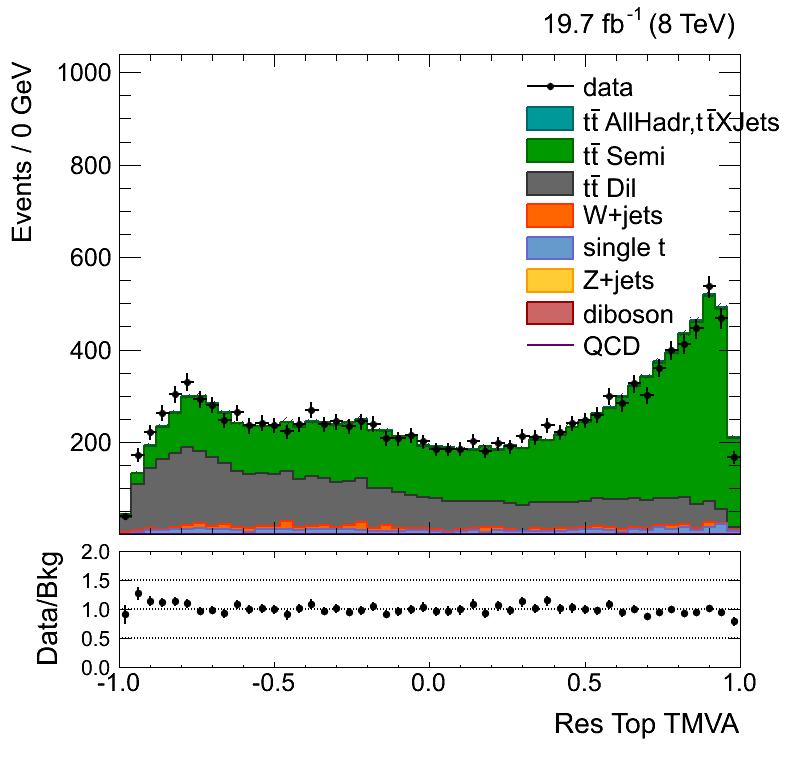
\includegraphics[width=0.48\textwidth]{figures/semilep_1tightmuo_resolved_3ormorejets_2ormorejetWPm_pfmetmore100_pfmtmore40_trigrequestonMC_17102015/hResTopMVAlinear.png}
	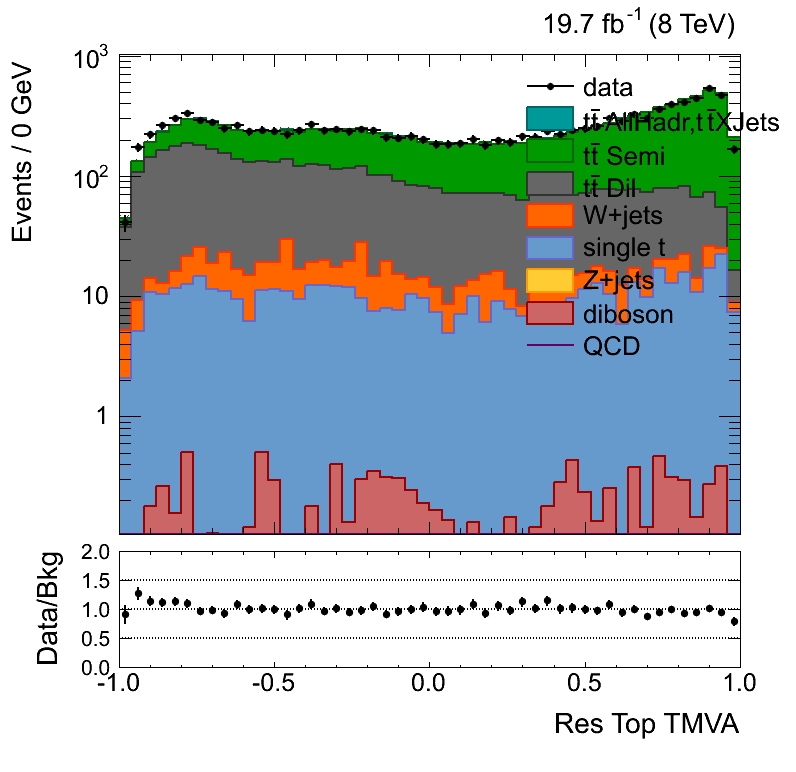
\includegraphics[width=0.48\textwidth]{figures/semilep_1tightmuo_resolved_3ormorejets_2ormorejetWPm_pfmetmore100_pfmtmore40_trigrequestonMC_17102015/hResTopMVA.png}
	\caption{Resolved top tagger MVA output score distributions in data and MC in linear and log scale}
	\label{fig:score}
\end{figure}


 \begin{figure}[htbp]
	\centering
	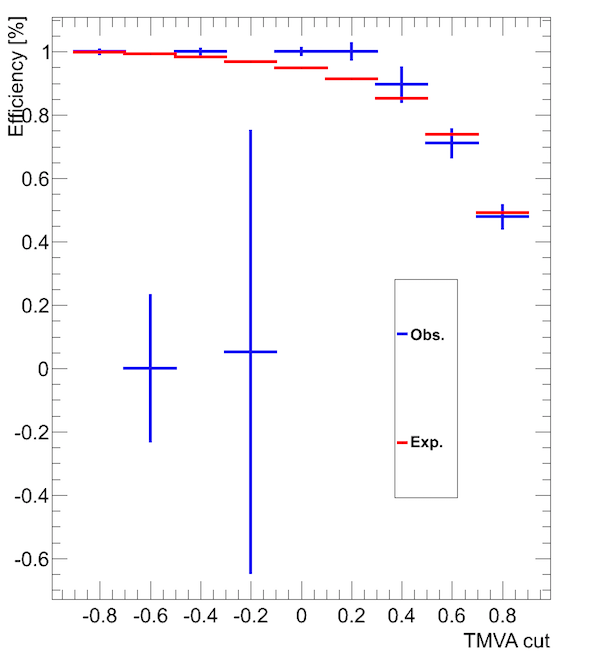
\includegraphics[width=0.48\textwidth]{figures/TOPRESOLVEDTAGGER/c_eff.png}\\
	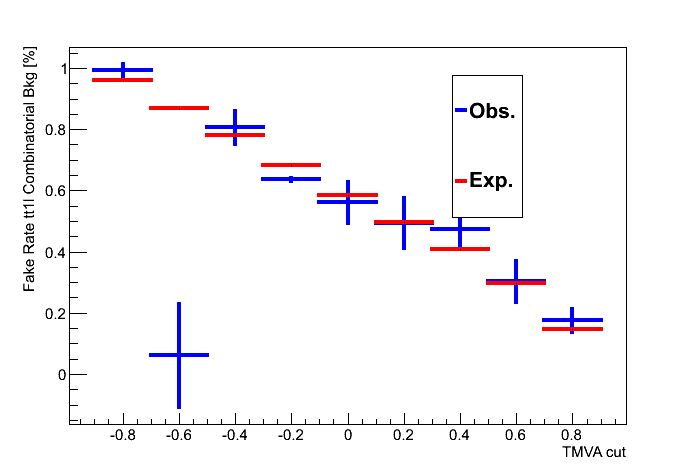
\includegraphics[width=0.48\textwidth]{figures/TOPRESOLVEDTAGGER/c_fr1.png}
	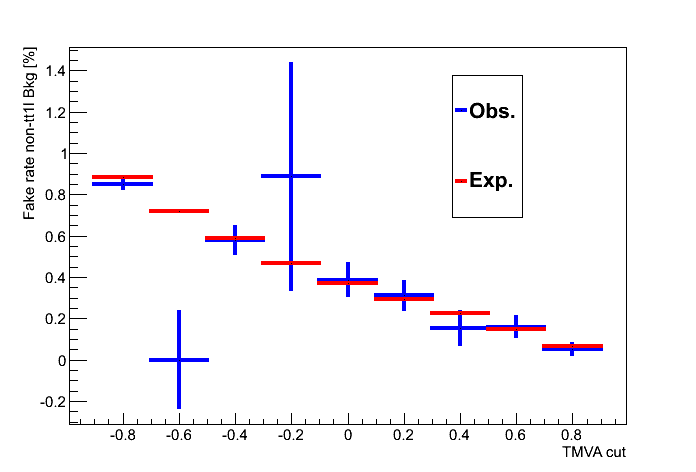
\includegraphics[width=0.48\textwidth]{figures/TOPRESOLVEDTAGGER/c_fr2.png}
	\caption{Signal efficiency (top),  combinatorial background fake rate (bottom left), and non-$\ttbar(1\Lep)$ background fake rate (bottom right) in 8 TeV data (blue) and mc (red) as function of the MVA threshold. The procedure to estimate those quantities has been described in the text. For the few bins where data and the predictions are consistent we noticed that Roofit has not reached convergence. \textcolor{red}{TO BE UNDERSTOOD}}
	\label{fig:roofitresults13TeV}
\end{figure}